\section{Smart Owl}
  \subsection{Definición}
  \paragraph{La función principal del Smart Owl es obtener información de diversas fuentes que proveen datos climáticos y de contaminación y exponer esta información de manera estandarizada con una estructura definida en formato JSON (véase Figura 8.7).}
  \begin{figure}[h!]
    \centering
      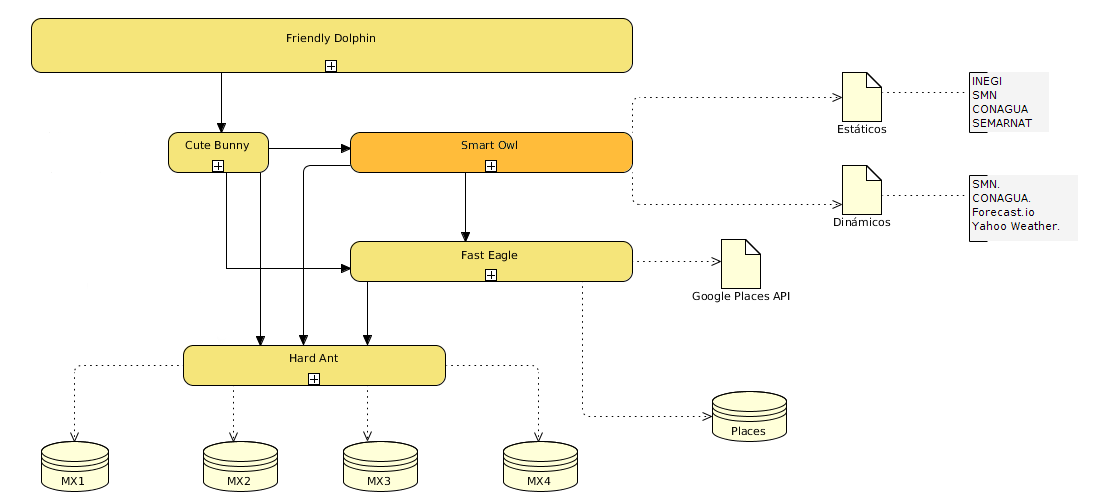
\includegraphics[width=\textwidth]{./images/DiagramaAmbienta2MX_SmartOwl.png}
    \caption{Smart Owl, Modulo de Ambienta2MX.} 
  \end{figure}
  \paragraph{Todas la información que se encontrará en las bases de datos de tipo MX será obtenida a través de Smart Owl, muchas de las fuentes no cuentan con los datos climatológicos completos, principalmente las gubernamentales como: CONAGUA, INEGI o SMN, por citar algunas.}
  \paragraph{Considerando esa problematica, Smart Owl busca y trata de resolver la información de los campos faltantes tomando como base distintas fuentes de datos, algunas establecidas y otras de tipo gubernamental.}
  \paragraph{También se tomará información de fuentes que tipo dinámica,es decir, cuya información suele ser actualizada en entre periodos de una o dos horas. Estas fuentes suelen contar con RESTFul API's para consumo de forma programática.}
  \paragraph{El modelo de datos final podrá ser entonces persistido después de que haya sido resuelto completa o parcialmente la petición.} 
  \paragraph{Se llevará el control de los metadatos considerando su origen, su fecha y algunos tags relacionados los que proveen la información.}
  \newpage

  \subsection{Alcances}
  
    \paragraph{Una vez que se definieron las fuentes principales para la obtención de datos se escribió una prueba que verifica la obtención de la información de cada una de ellas.} 
    \paragraph{La primera fuente de la que se extrajo información fueron los archivos que publica cada 10 minutos la página de la CONAGUA en el sitio \textbf{http://smn.cna.gob.mx/emas/}.}
    \paragraph{La técnica de Web Scraping fue utilizada para la extracción de los archivos que generan las diferentes estaciones ubicadas en los estados de las república (véase Figura 8.8).}
    \paragraph{Para ello se busco la url de cada archivo generado en todas las estaciones del país con ayuda de la biblioteca \textbf{tagsoup}.}
    \paragraph{Después de obtener las urls se persistieron en una base de datos no relacional de tipo llave-valor, en donde la llave es el valor de la latitud y longitud de la estación que genera la información}
    \begin{figure}[b!]
      \begin{center}
        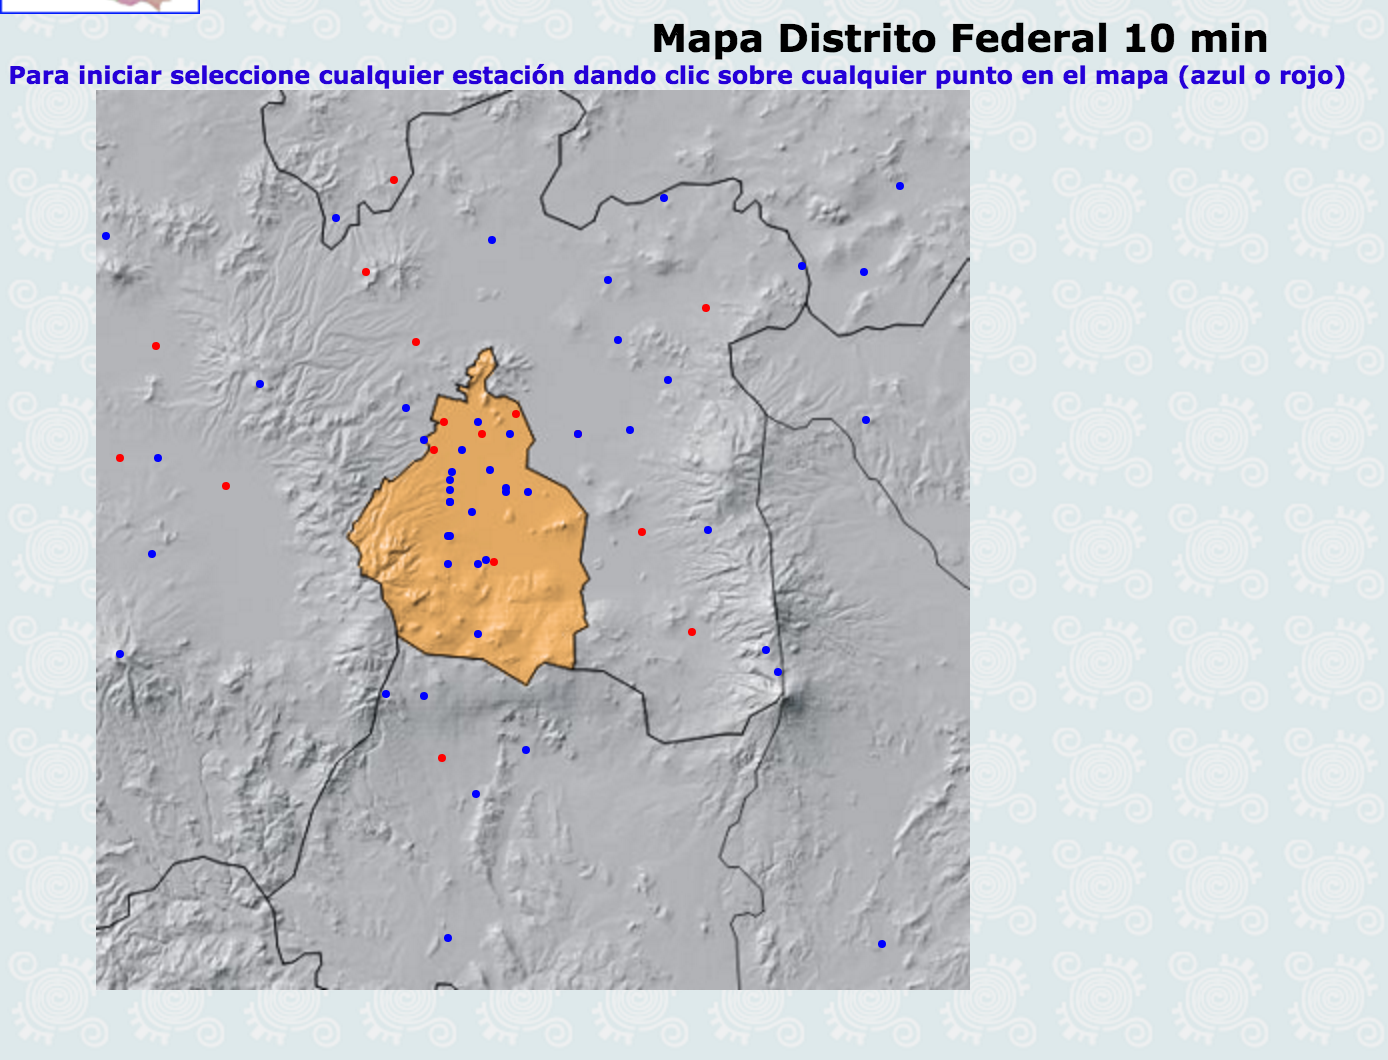
\includegraphics[width=14cm,height=10cm]{./images/DF_Stations}
        \caption{Estaciones con información climática del Distrito Federal}
      \end{center}
    \end{figure}
    \paragraph{Este proceso se ejecuta una sola vez en la aplicación, ya que cuando se despliega se verifica que ya existan las urls de los archivos en la base de datos}
    \paragraph{Ya que se tienen la información de los archivos disponible, se toma busca en la base la url del que tenga la latitud y longitud más cercana a los parámetros de consulta de la API para descargarlo y posteriormente iniciar el proceso extracción de las variables} 
    \paragraph{La segunda fuente con la que se intenta complementar el modelo es Weather Underground.}
  \paragraph{Este sitio expone un servicio que recibe un código de ciudad para obtener la información climática (véase Figura 8.9).}
    \begin{figure}[b!]
      \centering 
      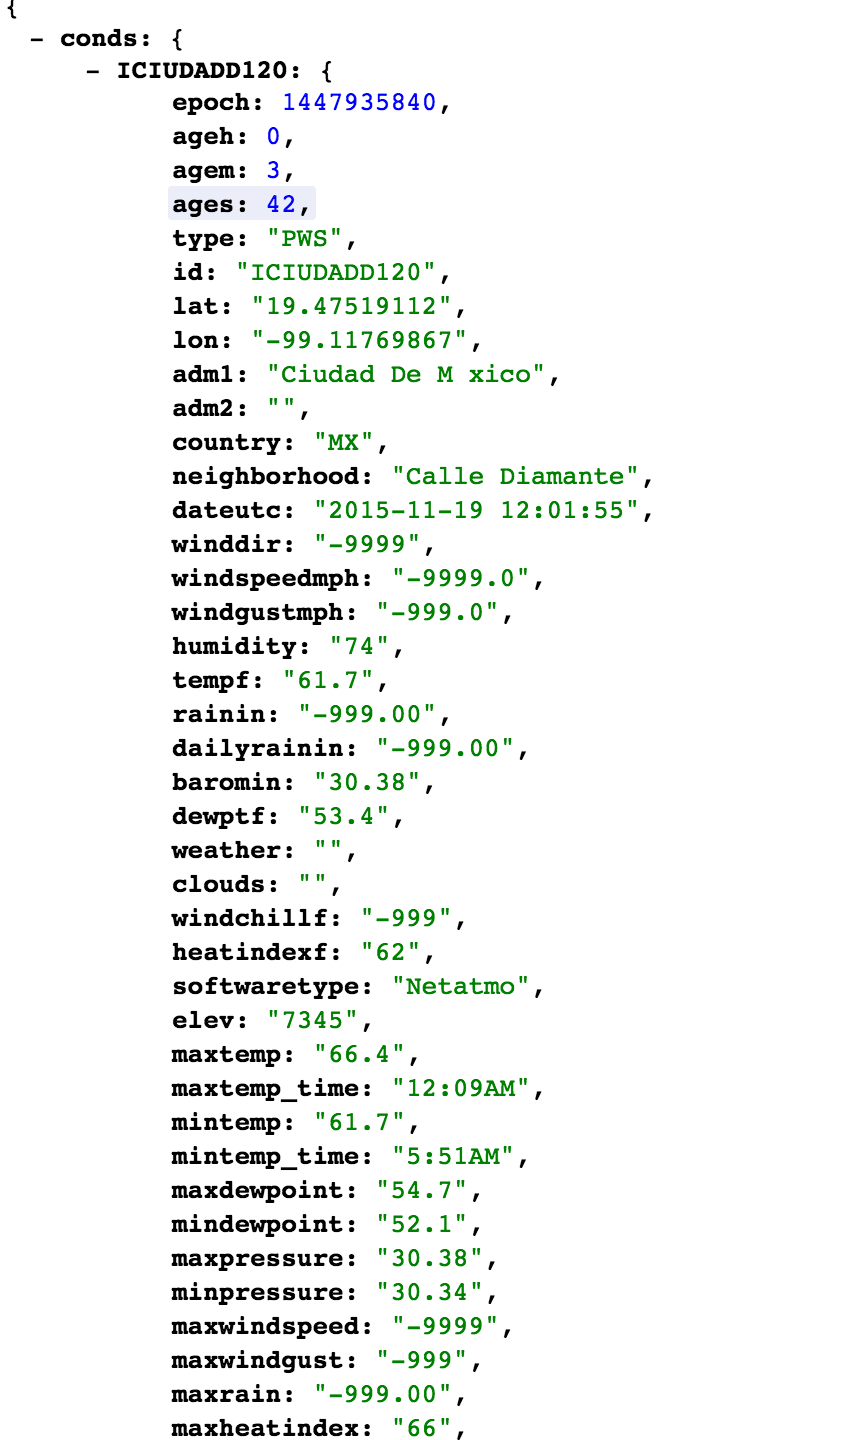
\includegraphics[width=12cm,height=12cm]{./images/WeatherUnderground}
      \caption{Consulta al servicio de WeatherUnderground}
    \end{figure}
  \paragraph{Finalmente, si el modelo de datos aún no está completo, se consulta a la API de Forecast.io para buscar los datos faltantes. Esta es la última opción de búsqueda ya que la API tiene un número limitado de consultas por día.}
  \newpage
  
  \subsection{Restricciones}
    \paragraph{En algunas ocasiones no será posible encontrar toda la información climática o de contaminación.}
    \paragraph{El funcionamiento del módulo depende de las fuentes de información disponibles, por lo que si alguna falla o no está disponible no será posible mostrar correctamente la información.}
    \paragraph{Si el formato de los archivos de la CONAGUA cambia también ocurrirán errores en la aplicación, sin embargo hay pocas probabilidades de que esto ocurra.}

  \subsection{Arquitectura}
    \paragraph{El módulo se realizó pensando en una arquitectura orientada a Microservicios.}
    \paragraph{Smart Owl es un microservicio que se despliega con un Tomcat embebido y expone la información siguiendo las convenciones de una aplicación REST.}

    \paragraph{El siguiente diagrama de clases muestra el modelo que define el estándar de los datos.}
    \begin{figure}[b!]
      \begin{center}
        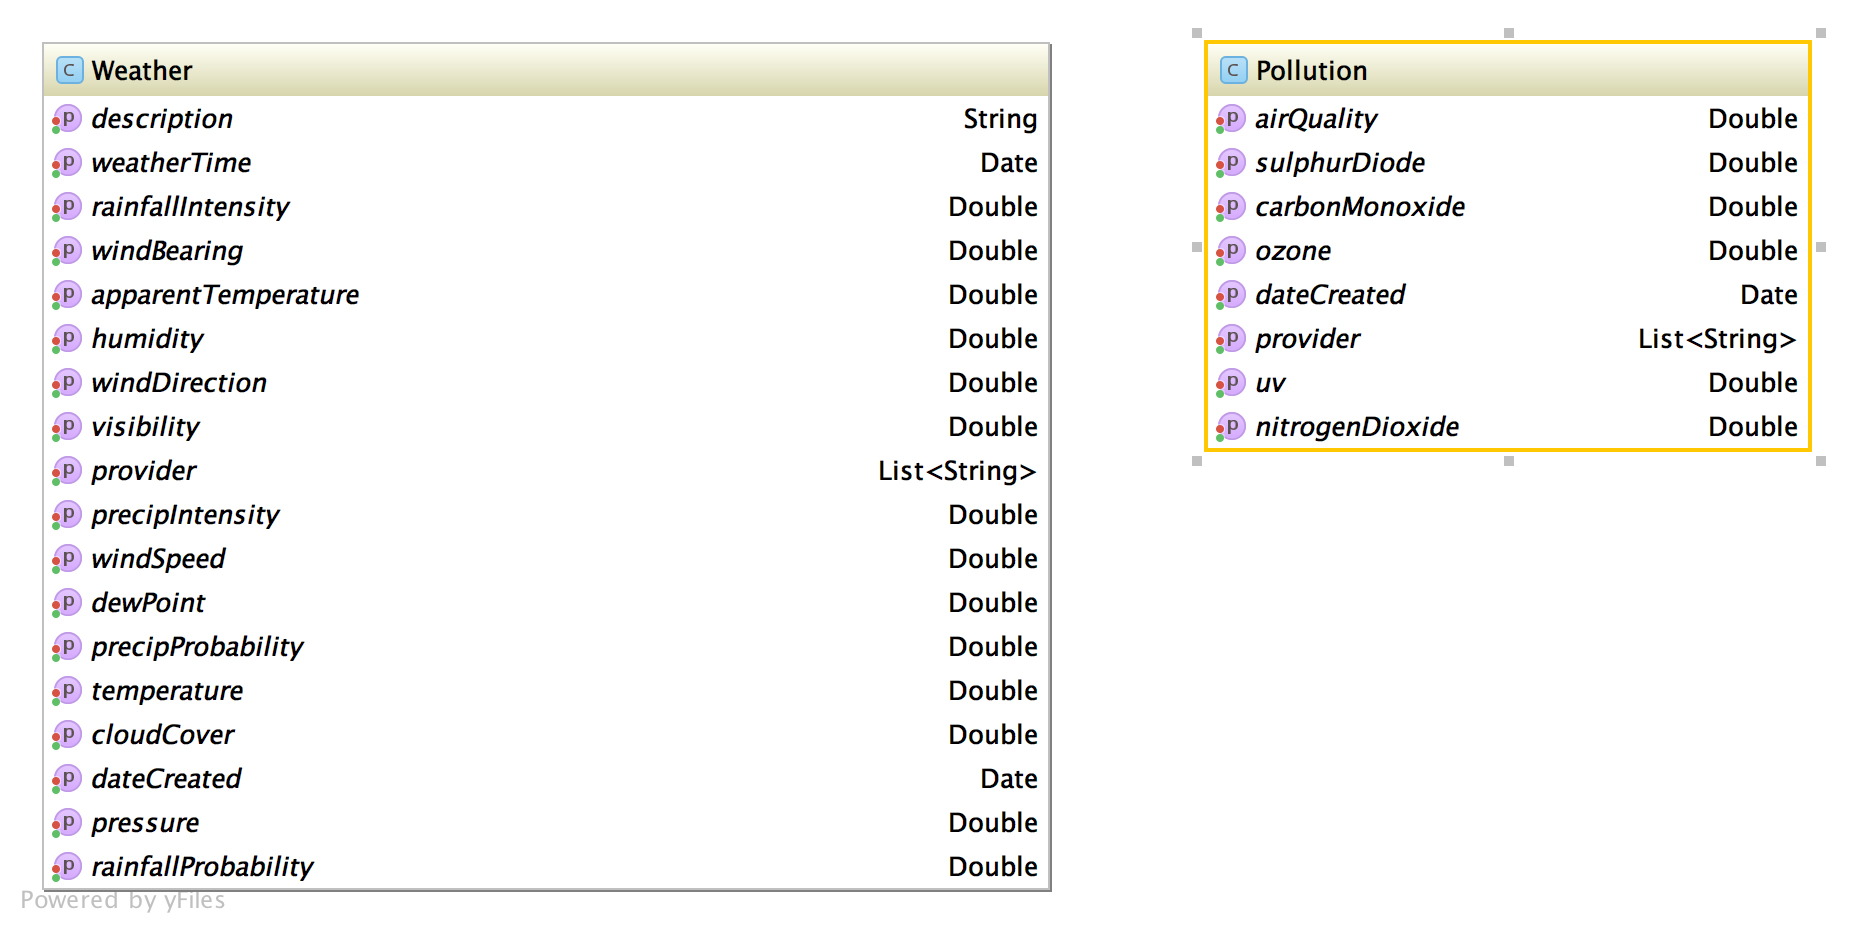
\includegraphics[width=14cm,height=10cm]{./images/SmartOwl_ClassDiagram}
        \caption{Diagrama de clases}
      \end{center}
    \end{figure}
    \paragraph{A continuación se muestran los diagramas de secuencia planteados para el funcionamiento del módulo mencionado.}

    \begin{figure}[b!]
      \begin{center}
        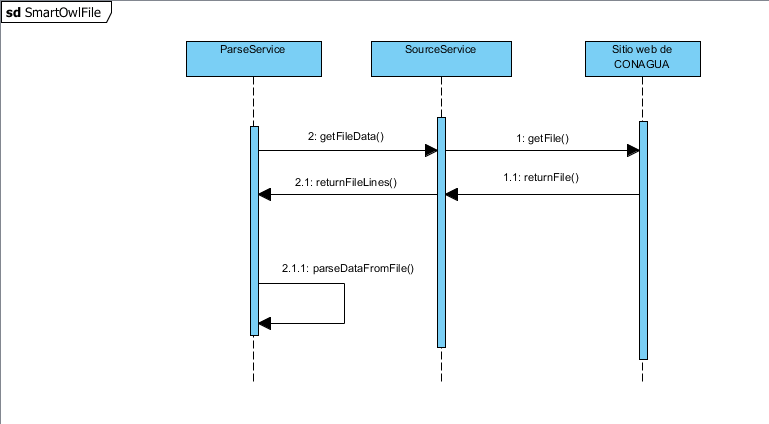
\includegraphics[width=14cm,height=9cm]{./images/SmartOwlSequenceDiagram}
      \end{center}
    \end{figure}

    \begin{figure}[b!]
      \begin{center}
        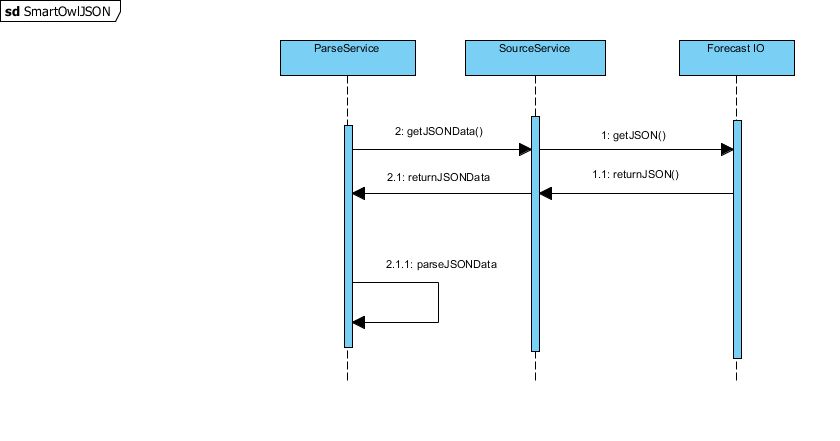
\includegraphics[width=14cm,height=9cm]{./images/SmartOwlSequenceDiagram2}
      \end{center}
    \end{figure}

  \subsection{Estudio de Factibilidad}
    \paragraph{El desarrollo de la aplicación es posible ya que existen fuentes gratuitas que proveen la información necesaria para completar el modelo de datos que quiere exponerse y estandarizarse.}

    \paragraph{Las fuentes para la construcción de la API son las siguientes:} 
    \begin{itemize}
      \item Archivos de texto de texto que provee la CONAGUA (Comisión Nacional del Agua) con información climática
      \item Información de la página de Weather Underground
      \item API de Forecast.io
    \end{itemize}
    
    \paragraph{Hubo complejidad en la obtención de los datos ya que las fuentes presentan estructuras muy variadas, sin embargo, con ayuda de las pruebas unitarias fue posible implementar la funcionalidad para llenar el modelo de datos propuesto de manerá sencilla.}
  
  \subsection{Implementación}
  \paragraph{Para el desarrollo del módulo se hizo uso del lenguaje de programación Groovy.} 

  \paragraph{Smart Owl es un microservicio que se despliega con ayuda de SpringBoot y expone dos urls: /weather y /pollution que reciben los parámetros \textbf{latitude} y \textbf{longitude} para la búsqueda de la información.}

  \paragraph{Se escribió un conjunto de pruebas unitarias para la funcionalidad de la obtención de datos y la estandarización de la información con la ayuda de Spock Framework.}

  \paragraph{Gradle fue útli para las tareas de testing, administración de dependencias y la implementación del framework SpringBoot para el despliegue de la aplicación.}

  \subsection{Pruebas}
  \begin{figure}[b!]
      \begin{center}
        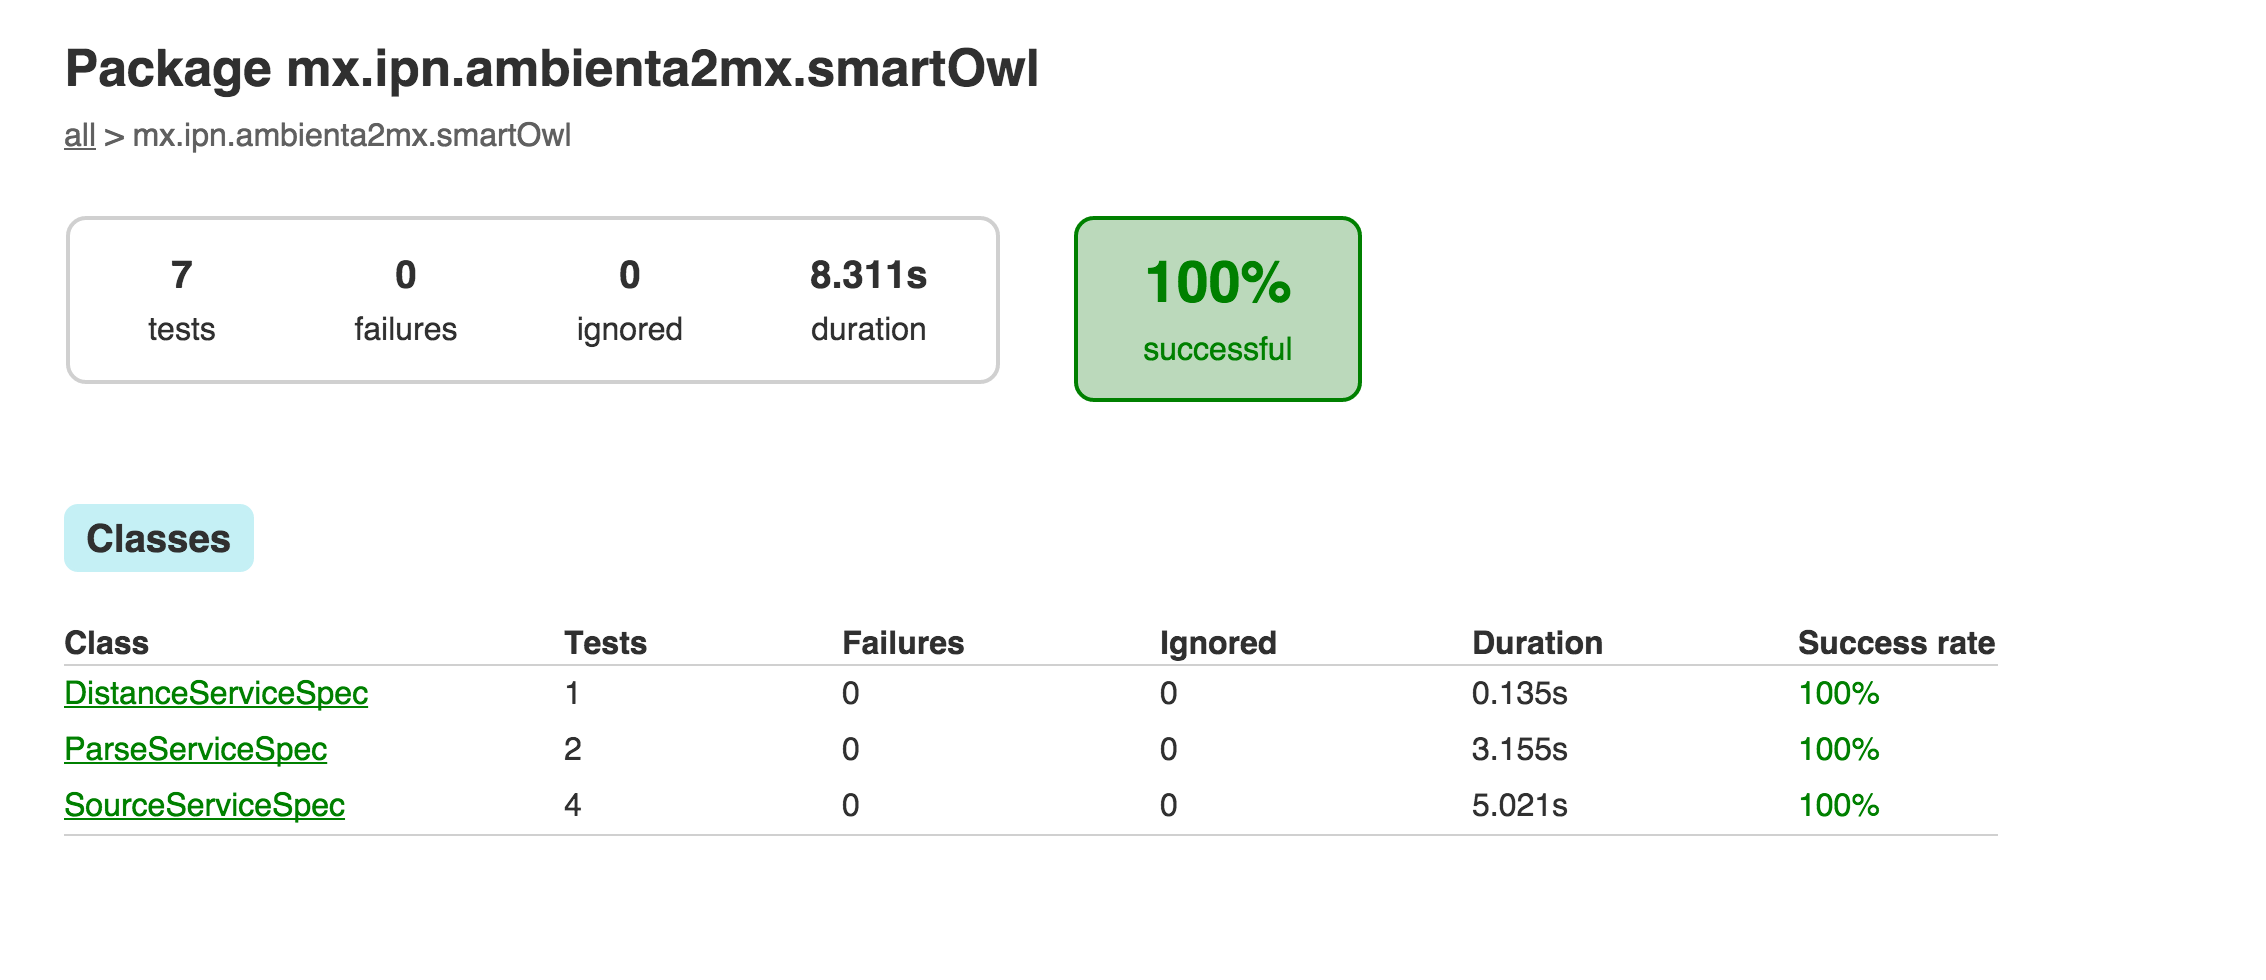
\includegraphics[width=14cm,height=9cm]{./images/prueba1}
      \end{center}
    \end{figure}
    \begin{figure}[b!]
      \begin{center}
        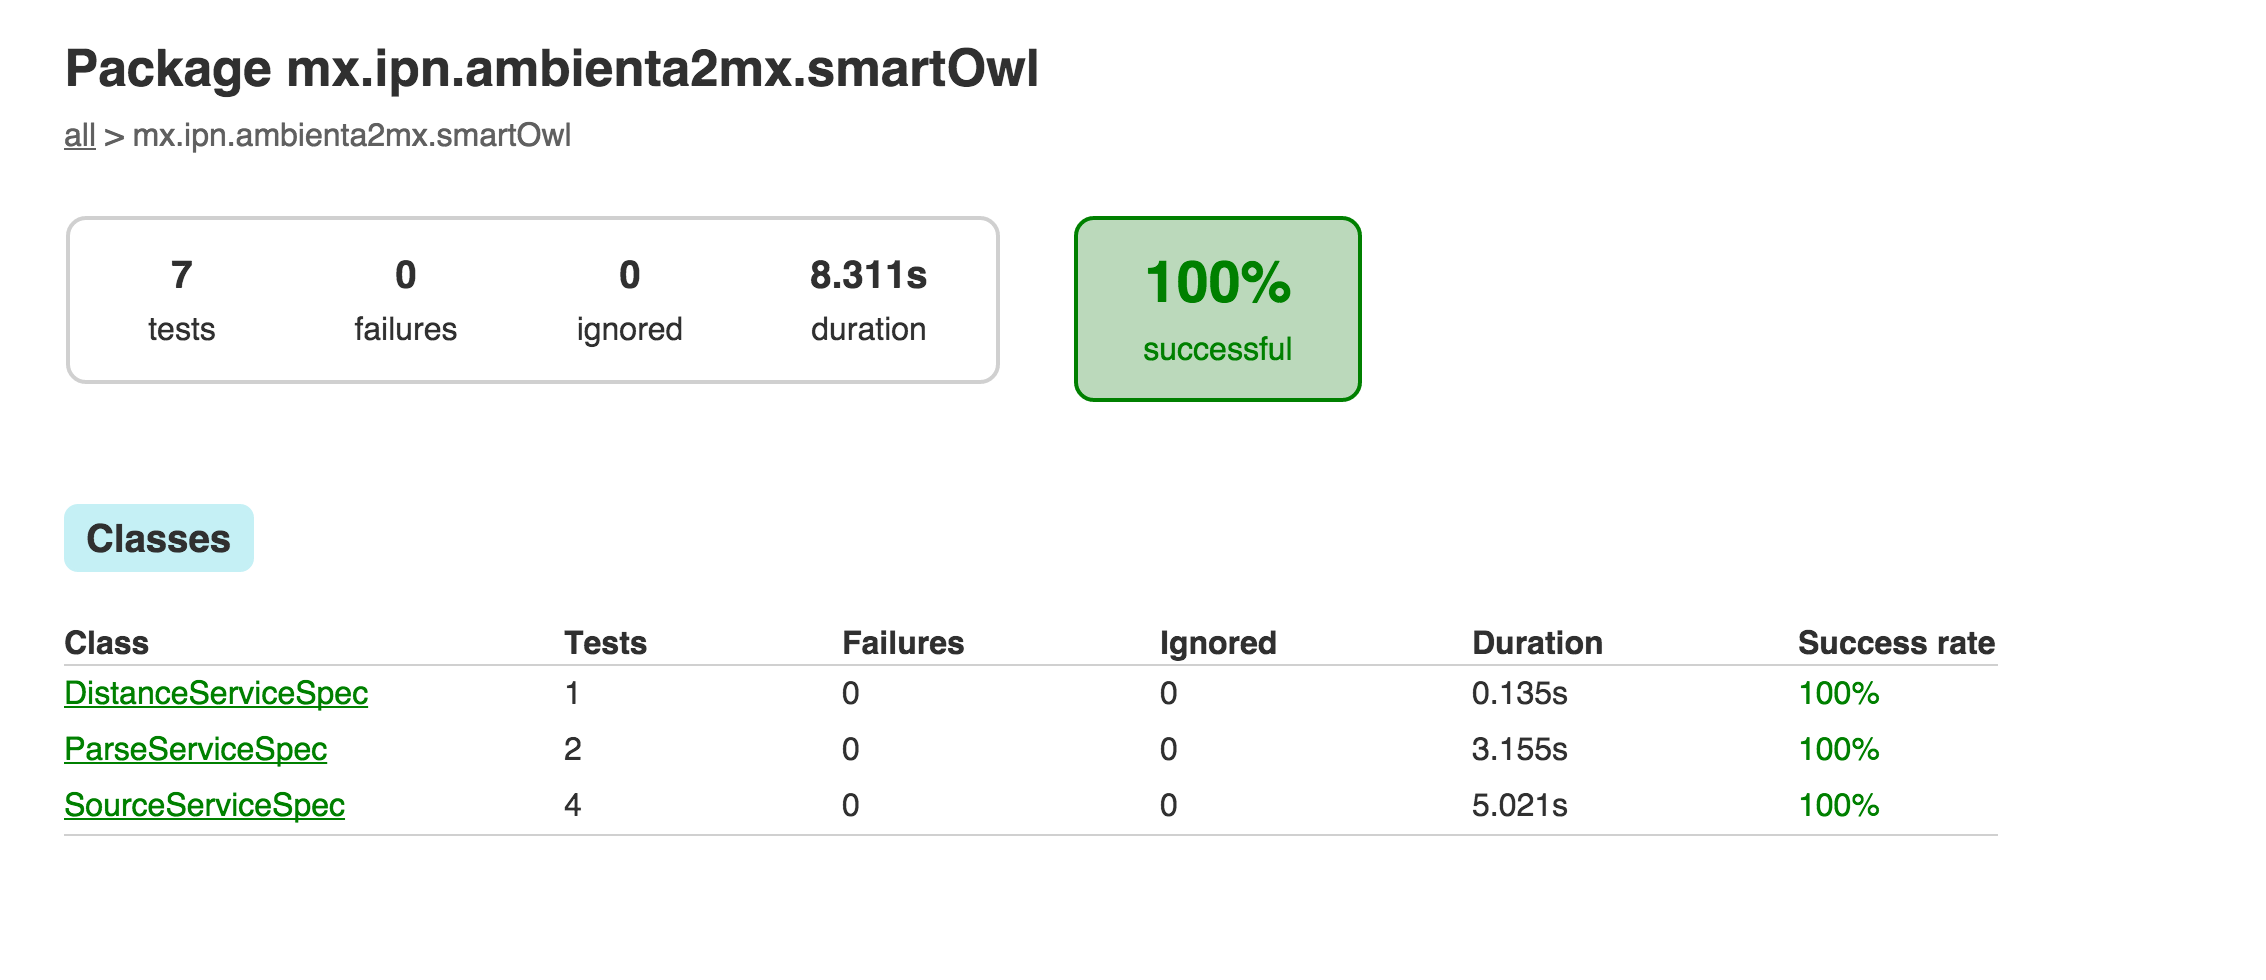
\includegraphics[width=14cm,height=9cm]{./images/prueba1}
      \end{center}
    \end{figure}
    \begin{figure}[b!]
      \begin{center}
        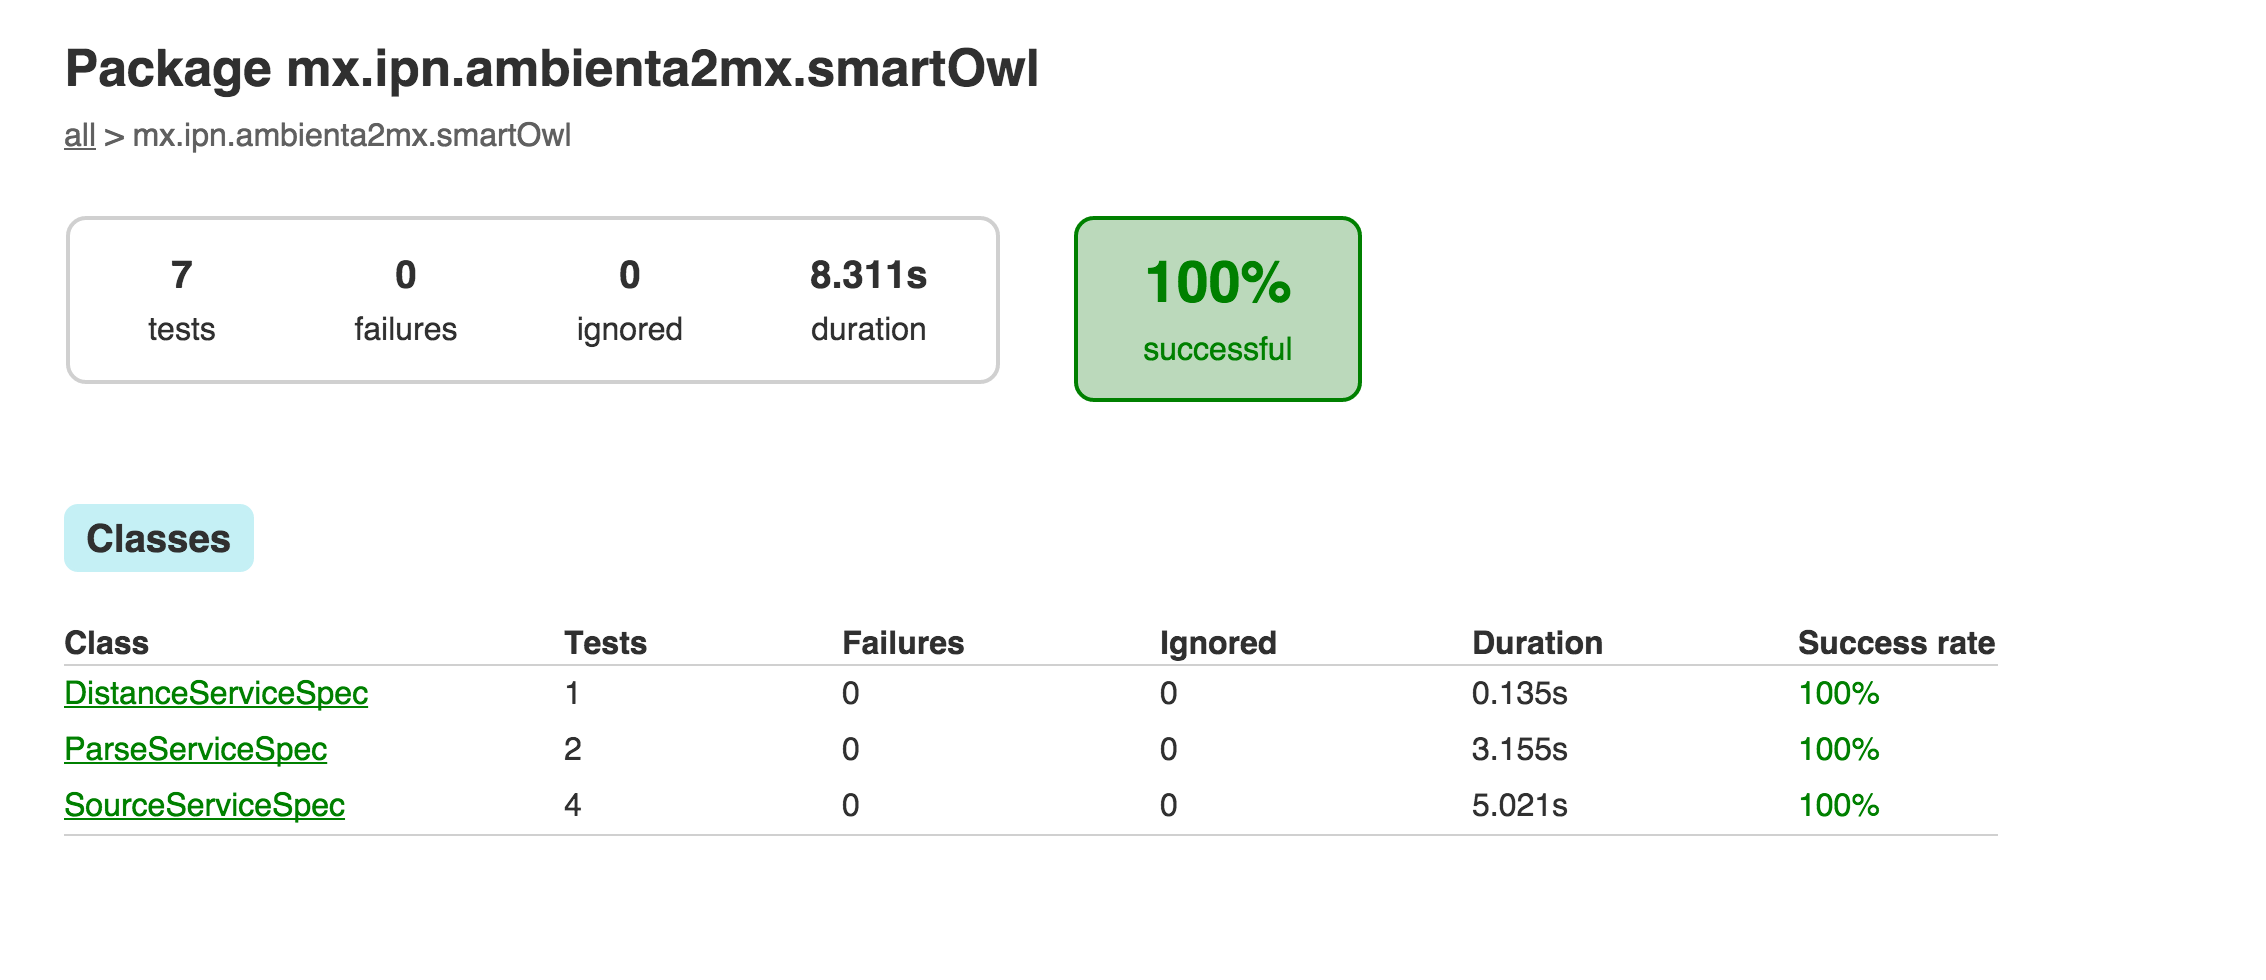
\includegraphics[width=14cm,height=9cm]{./images/prueba1}
      \end{center}
    \end{figure}
    \begin{figure}[b!]
      \begin{center}
        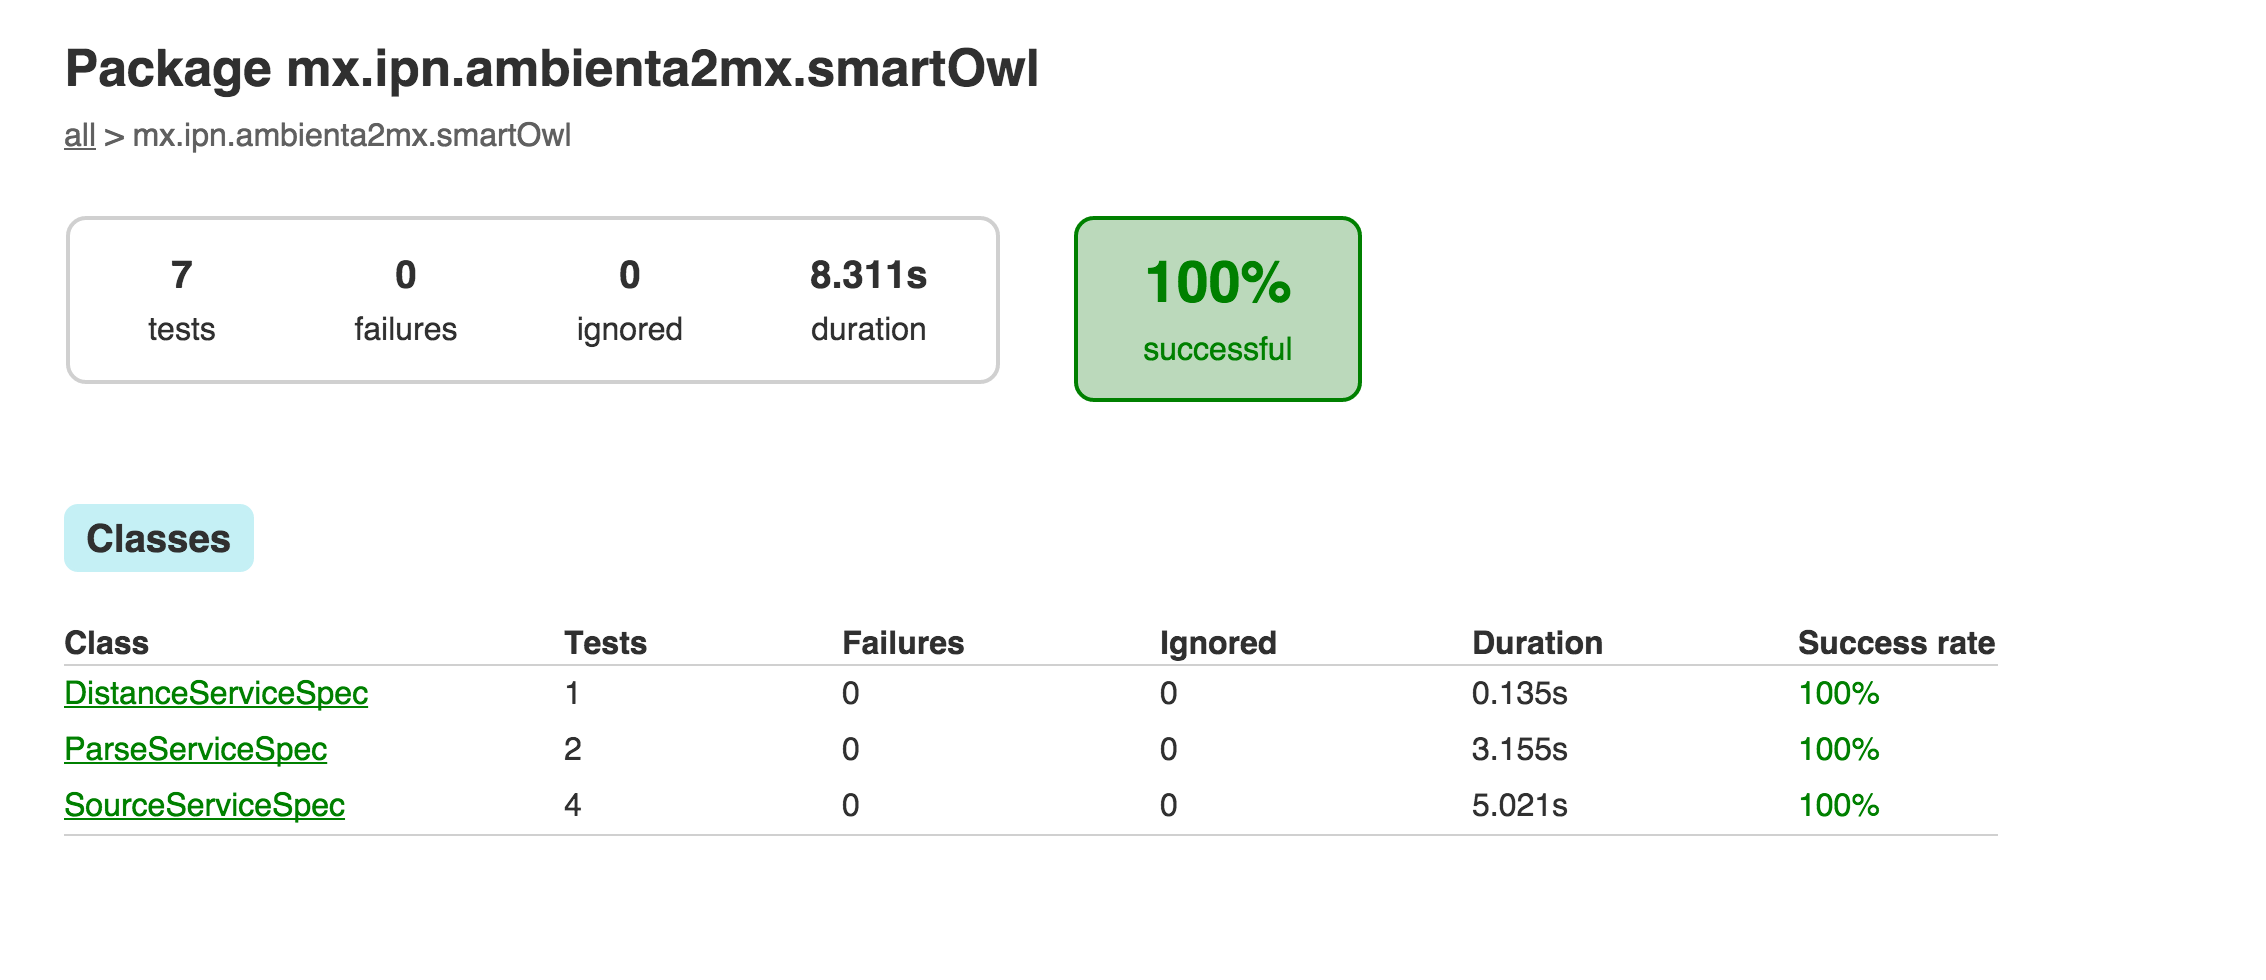
\includegraphics[width=14cm,height=9cm]{./images/prueba1}
      \end{center}
    \end{figure}
